\documentclass[12pt,a4paper]{article}

%  PACKAGES
%Basic Text
\usepackage[latin1]{inputenc}
\usepackage{amsmath}
\usepackage{amsfonts}
\usepackage{amssymb}

%Figures
\usepackage{graphicx}
\usepackage{float}
\usepackage{epstopdf}
\usepackage{caption}
\usepackage{subcaption}
%Wraparound for large images
\usepackage{wrapfig}

%Hyperlinks For References + Links
\usepackage{hyperref}

%Nice Code Layout 
\usepackage{listings}

%Useful Physics Formatters
\usepackage{hepnames}
\usepackage{siunitx}

%Test If Floats Will Fit Preemtively
\usepackage{lipsum}

%  TITLE + PAGE INFO

\usepackage[affil-it]{authblk}
%\usepackage[superscript,biblabel]{cite}
\usepackage[width=18.0cm, height=26.00cm]{geometry}
\title{Further analysis of the cross correlation method for the detection of North Korea tests}
\author{Gareth Bird \\ \href{mailto:gareth.bird@sjc.ox.ac.uk}{gareth.bird@sjc.ox.ac.uk}}
\affil{University of Oxford}

%  COMMANDS
\newcommand{\secref}[1]{Section \ref{#1} }
\newcommand{\figref}[1]{Figure \ref{#1} }
\newcommand{\tabref}[1]{Table \ref{#1} }
\newcommand{\xco}{\textit{xcorrobj.py}}

%  DOCUMENT
\begin{document}
\maketitle
\begin{abstract}
	
\end{abstract}
\section{Introduction}
	With data from lower altitude satellites, seismic activity has been linked to particle bursts in similar L shells. \cite{aleksandrin2003high}. In currently unpublished work, the methods for matching particle bursts has been modified to be used on public access gps electron count data with reasonable success. Further to this, Filip Wach observed that by taking cross correlation data for the raw signal between energy channels of the satellites results in anomalous values compared to background data (see \figref{fig:filipex}) but there was not any discussions as to why.\cite{filipwach2017}
	
	This work was undertaken as a continuation of Filip Wach's work with main objective of taking and testing these analysis methods further. The project also aimed to detect the events not previously detected if the method could be replicated.
	
	All code for the project insofar has been created using Python 2.7 with Jupyter notebooks with simple wget commands in ubuntu. There also exists a parallelised version of this method but they are currently not compatible with one another. All branches of the code can be found \href{https://github.com/fw14863/SP_2017/network}{here}.
	\begin{figure}
		\centering
		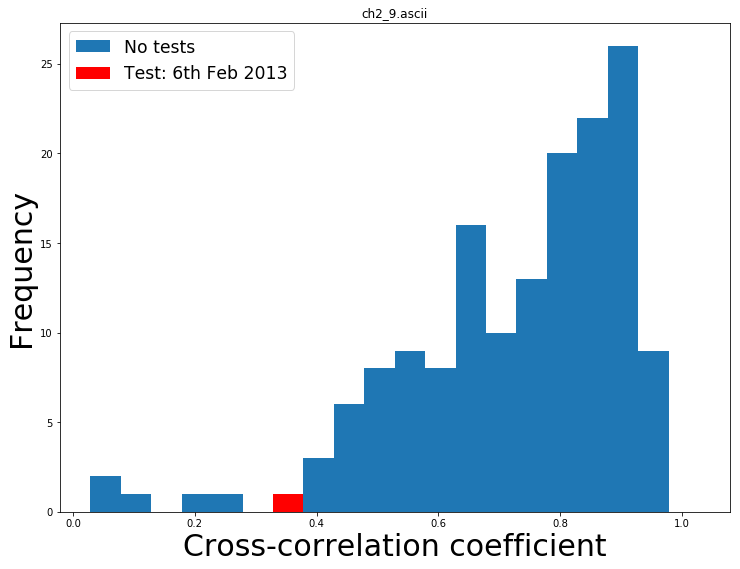
\includegraphics[width=0.6\linewidth]{Figures/filipex}
		\caption{An example plot of an outlying cross correlation value during a north korea test, taken from \cite{filipwach2017}}
		\label{fig:filipex}
	\end{figure}

	

	
\section{Methods}
	\subsection{Previous methodology modifications}\label{ssec:methmod}
	After tracing through the code from the previous project and discussing with group, a couple of a minor issues arose.
	\begin{itemize}
		\item
		When downloading data using the meta-search class, the data returned retrieved all file names between the given time interval, but did not then cut according to the dates provided. This seemed problematic as the background data did impose an exact time interval. As discussed later, this does have a effect on the cross correlation spectra (See Section \ref{ssec:Trends}) but does not invalidate the method.
		\item
		To modify the satellite number for downloading, the source code needed to modified and was not clearly labelled. This has been fixed in both new branches, with Jack's having more options.
		\item
		By inspection of the shape/size of the histogram, the background data sample size could have been larger
	\end{itemize}
	
	As a result the first job was to make the previous code replicable and clarifying the method further.
	  
	\subsection{General Procedure}
	All of my code involves analysing the data from the returned python dictionaries when calling the meta-search class method. This involves Further, the majority fo the code is finding and manipulating cross correlation values. This was done by splitting the data into equal time periods, calculating the cross correlation values and storing the information about the given time intervals alongside it. This allows me to generate the plots outlined in \secref{ssec:plotproc}.
	
	\subsection{General Object Structure}
	In an attempt to make my work easier to merge with other people's efforts, all my work is split into classes and methods within \textit{xcorrobj.py}.
	There are two main classes:
	\begin{enumerate}
		\item
		\textbf{crosscorrelator}: Its main function is to calculate cross correlations of raw electron count signals over given time intervals. Stores data and dates for a given interval.
		
		\item
		\textbf{plotgenerator}: Takes the satellite number and two instances of the correlator. Built to compare North Korea to Background data and save and repeat drawing instances of the data used in the plots.\footnote{A caveat is that not all the plot procedures are currently within plot generator although the code could easily be modified so that is the case.}
	\end{enumerate}
	\subsection{Plot procedures} \label{ssec:plotproc}
	The most instructive way to see all the plots generated  and to get an idea of structure is to look at the \textit{routine demonstrations} python notebooks for given satellites. The intended output of the plots methods are described in \tabref{tab:plotdesc}. For specific implementation information/ input arguments, please refer to the commented code within \xco. To save any particular plots to file instead of displaying, change the filename from an empty string.
	
	\begin{table}[h]
		\begin{tabular}{|l|p{0.6\linewidth}|}
			\hline
			\textbf{Method Name(s)} & \textbf{Description of output plot(s)}  \\ \hline
			 crosscorrelator.create\_NK\_plot & Recreates cross correaltion spectra plots in the same way as \figref{fig:filipex} but with the fixed time intervals. \\ \hline
			 crosscorrelator.createscatters &  A redundant method, replaced with generate\_signal\_time\_plots \\ \hline
			 plotgenerator.generate\_signal\_time\_plots& Generates scatters of plots with a range of cross correlation values for two channels with matching time series plots. Can also create matching fourier transforms and labels the scatters if they include bad data. \\ \hline
			 ...tor.generate\_bad\_data\_demonstration & Creates histograms of comparing the cross correlation values of intervals containing bad data labels in the sample interval file and  \\ \hline
			 fulldataconstruction or eventfinding & Generates a full set of cross correlation values for given intervals alongside finding when the minimum cross correlation value occurs in the North Korea data set and it's associated p value (proportion of background data smaller than the value) \\ \hline 
		\end{tabular}
		\caption{ Descriptions of the plot methods within \xco}
		\label{tab:plotdesc}
		\centering
	\end{table}
\section{Results}
This section is far from a complete set plots/deductions that can be found within the data files. Most of what is discussed in Sections \ref{ssec:Trends} and \ref{ssec:suggestions} arose from Skype discussion of the presentations. If you are continuing investigating these phenomena I'd recommend scanning through the extent of these plots yourself   \href{https://github.com/GarethBird96/SP_2017/tree/master/Presentations}{here}.
	\subsection{Plots and Trends}\label{ssec:Trends}
		\subsubsection{Further Cross Correlation Spectra Plots with timestamps (\textit{eventfinding})}
		\begin{figure}[h]
			\begin{subfigure}[b]{0.5\linewidth}
				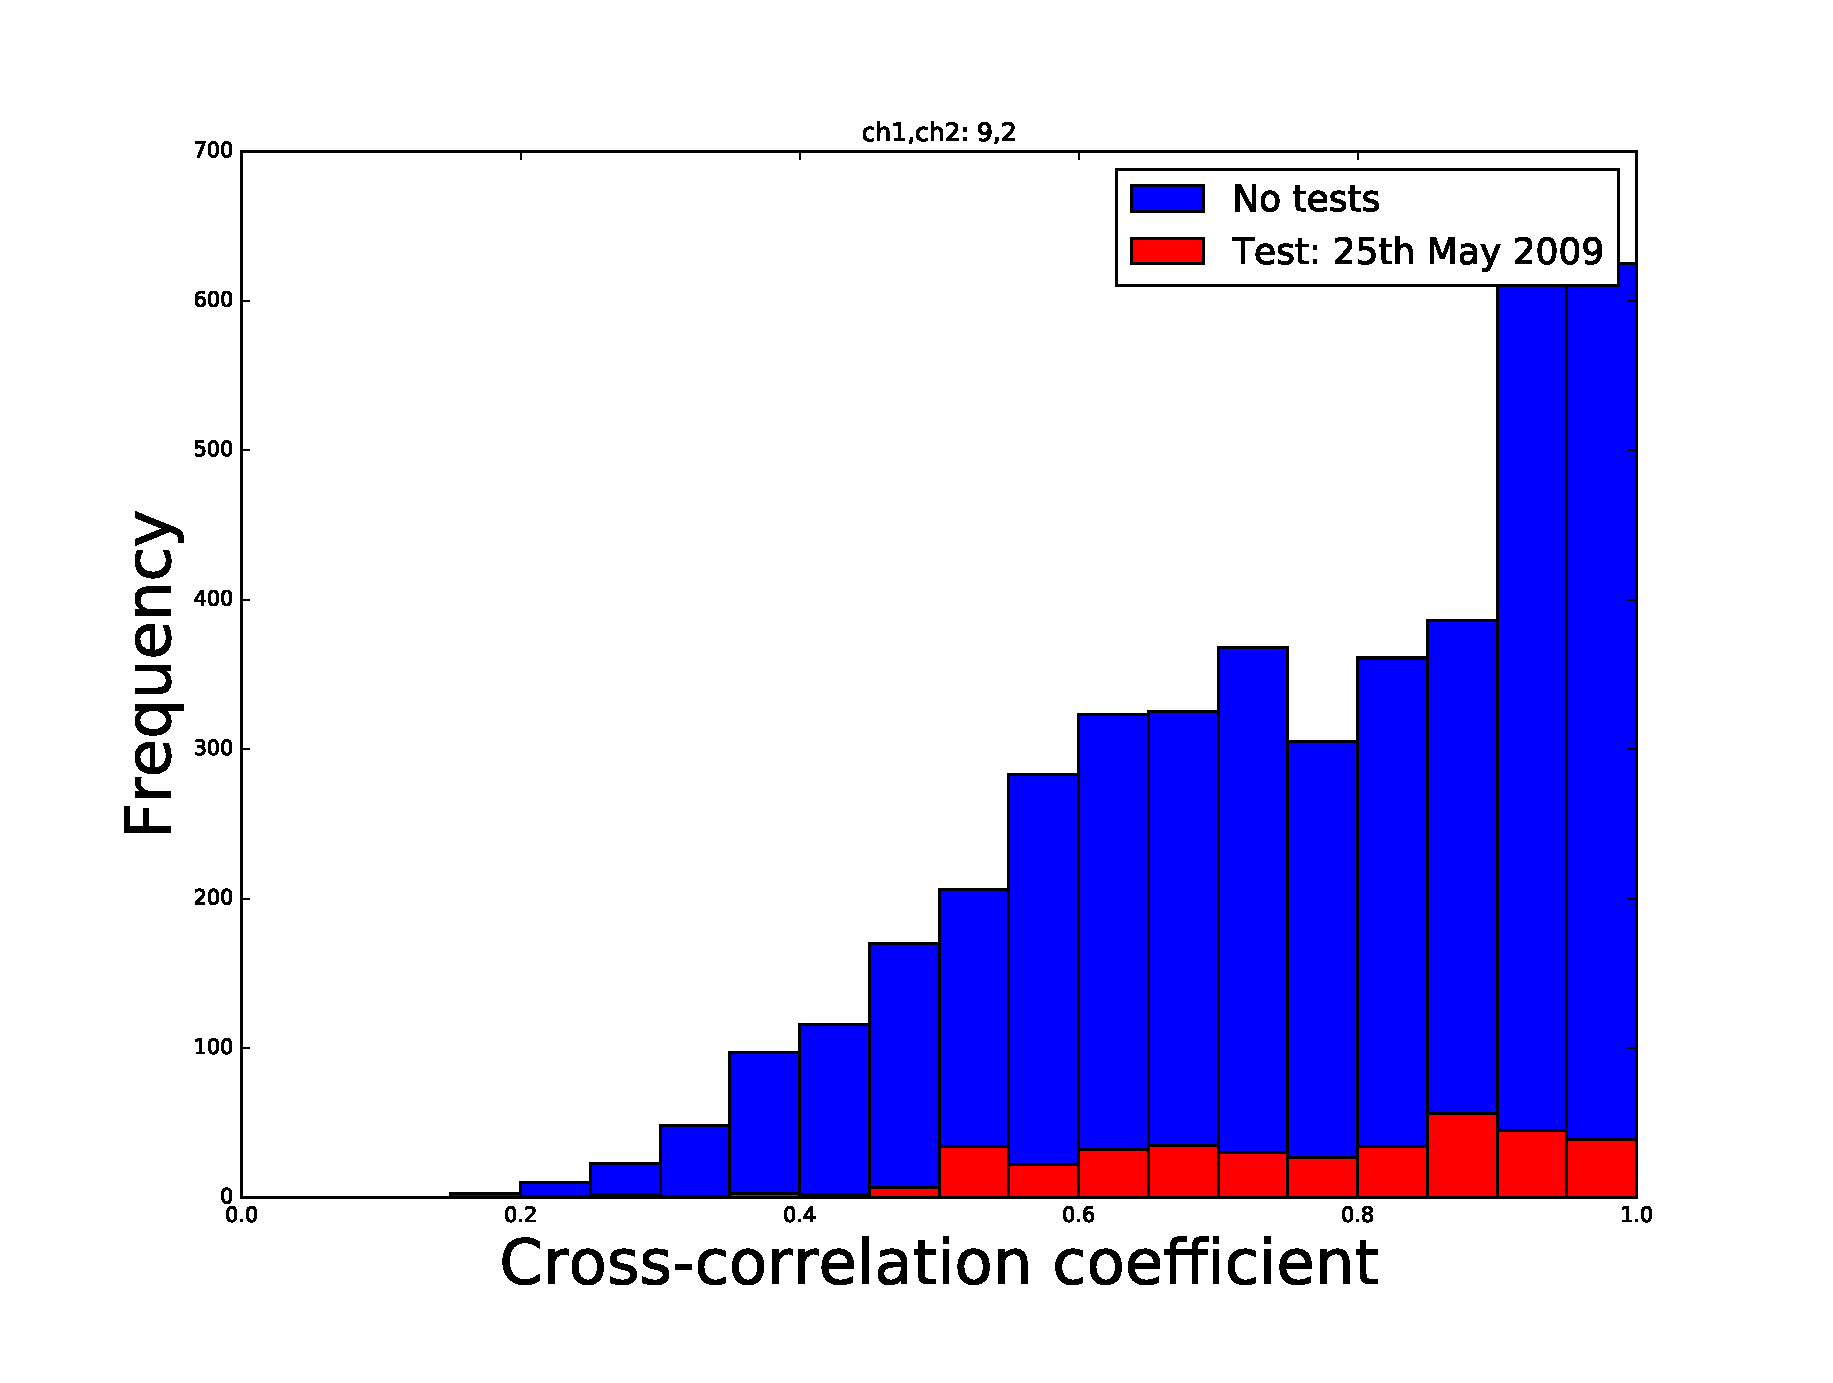
\includegraphics[width=\textwidth]{Figures/eventfind/4hours.eps}
				\caption{4 Hours}
			\end{subfigure}
			\begin{subfigure}[b]{0.5\linewidth}
				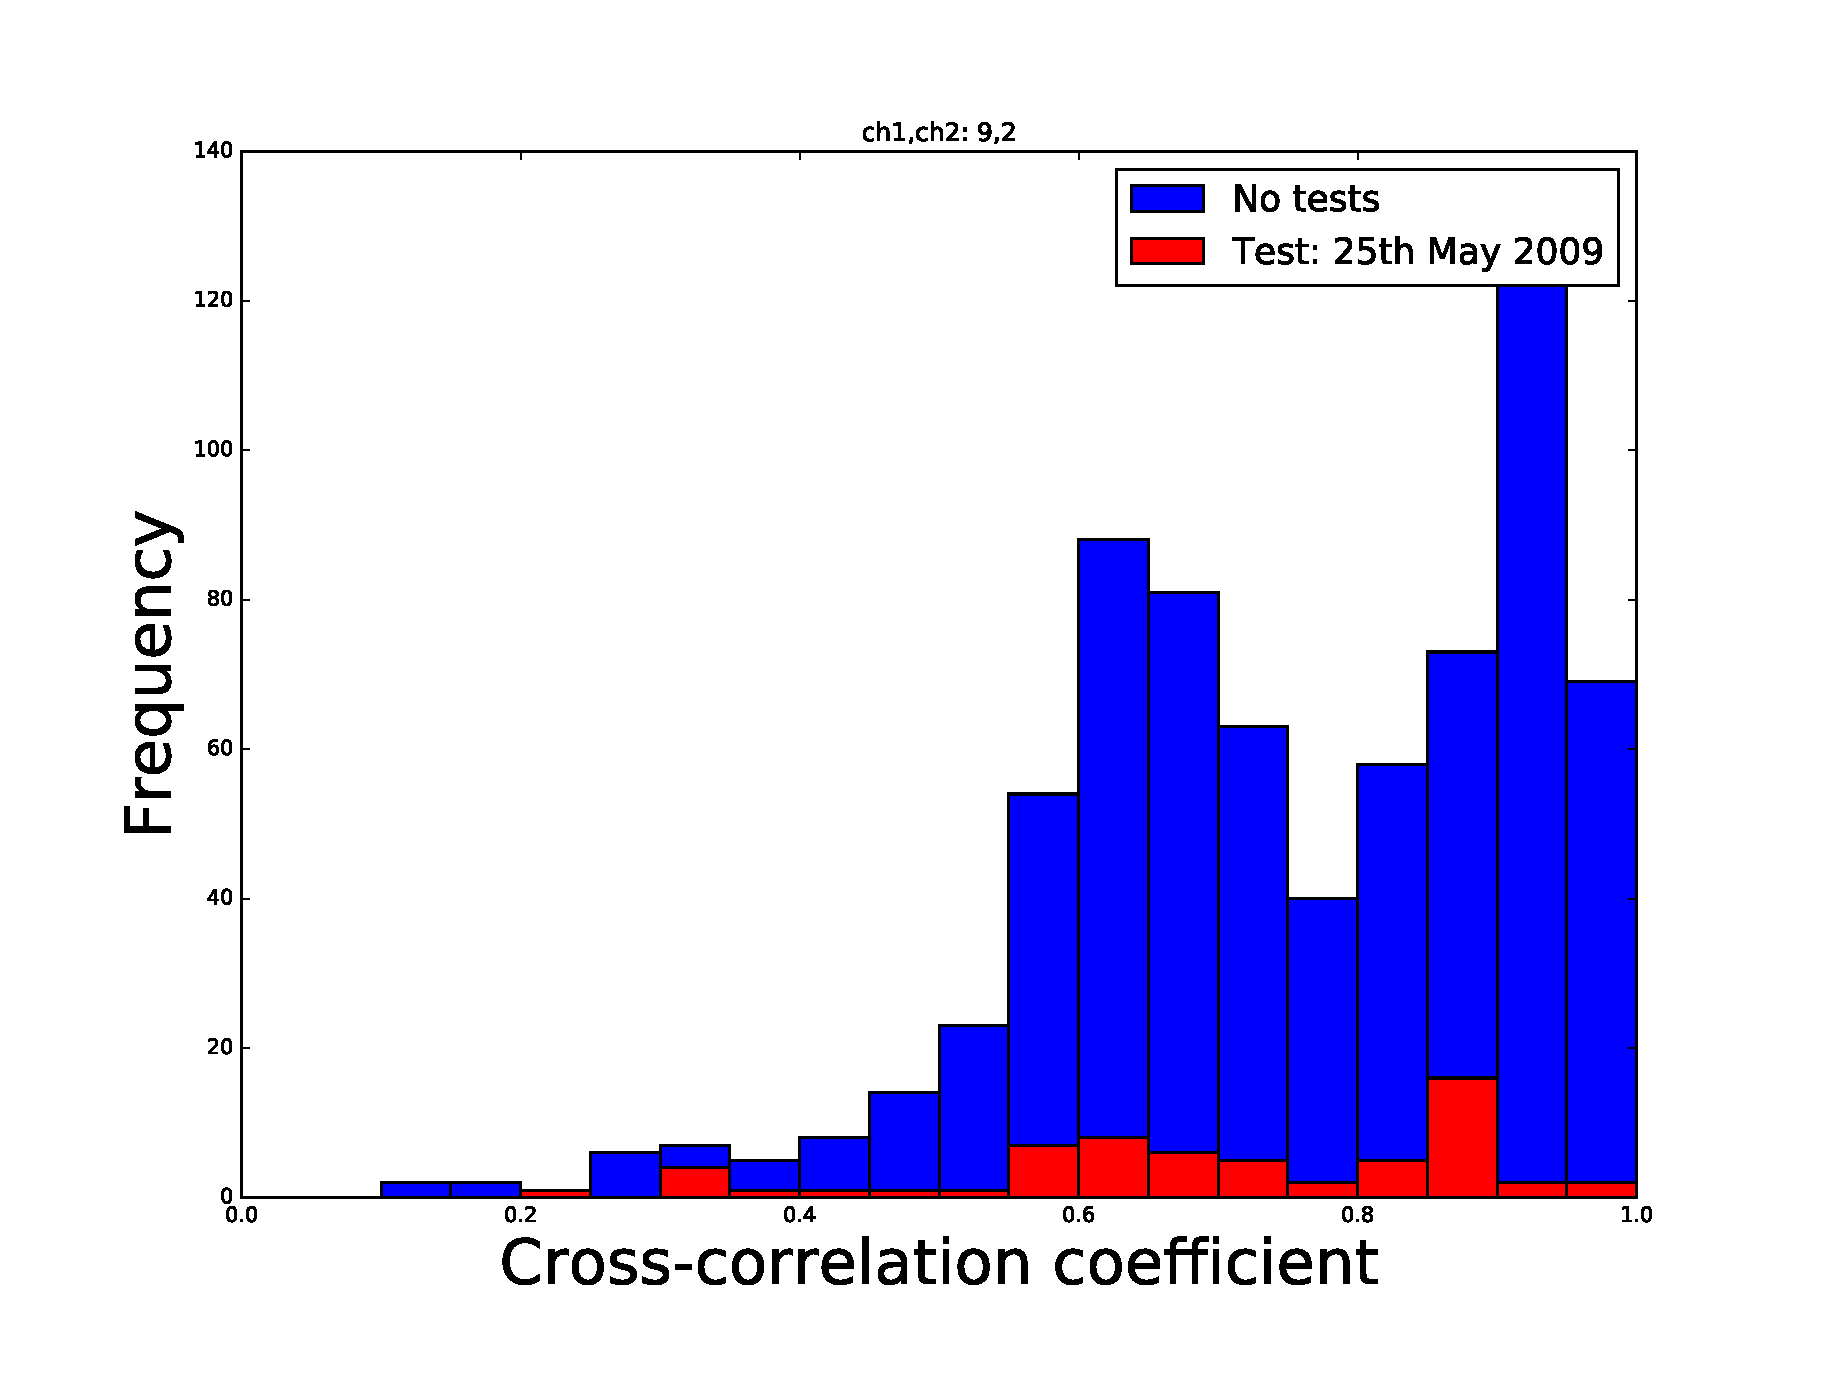
\includegraphics[width=\textwidth]{Figures/eventfind/24hours.eps}
				\caption{24 Hours}
			\end{subfigure}
			\begin{subfigure}[b]{0.5\linewidth}
				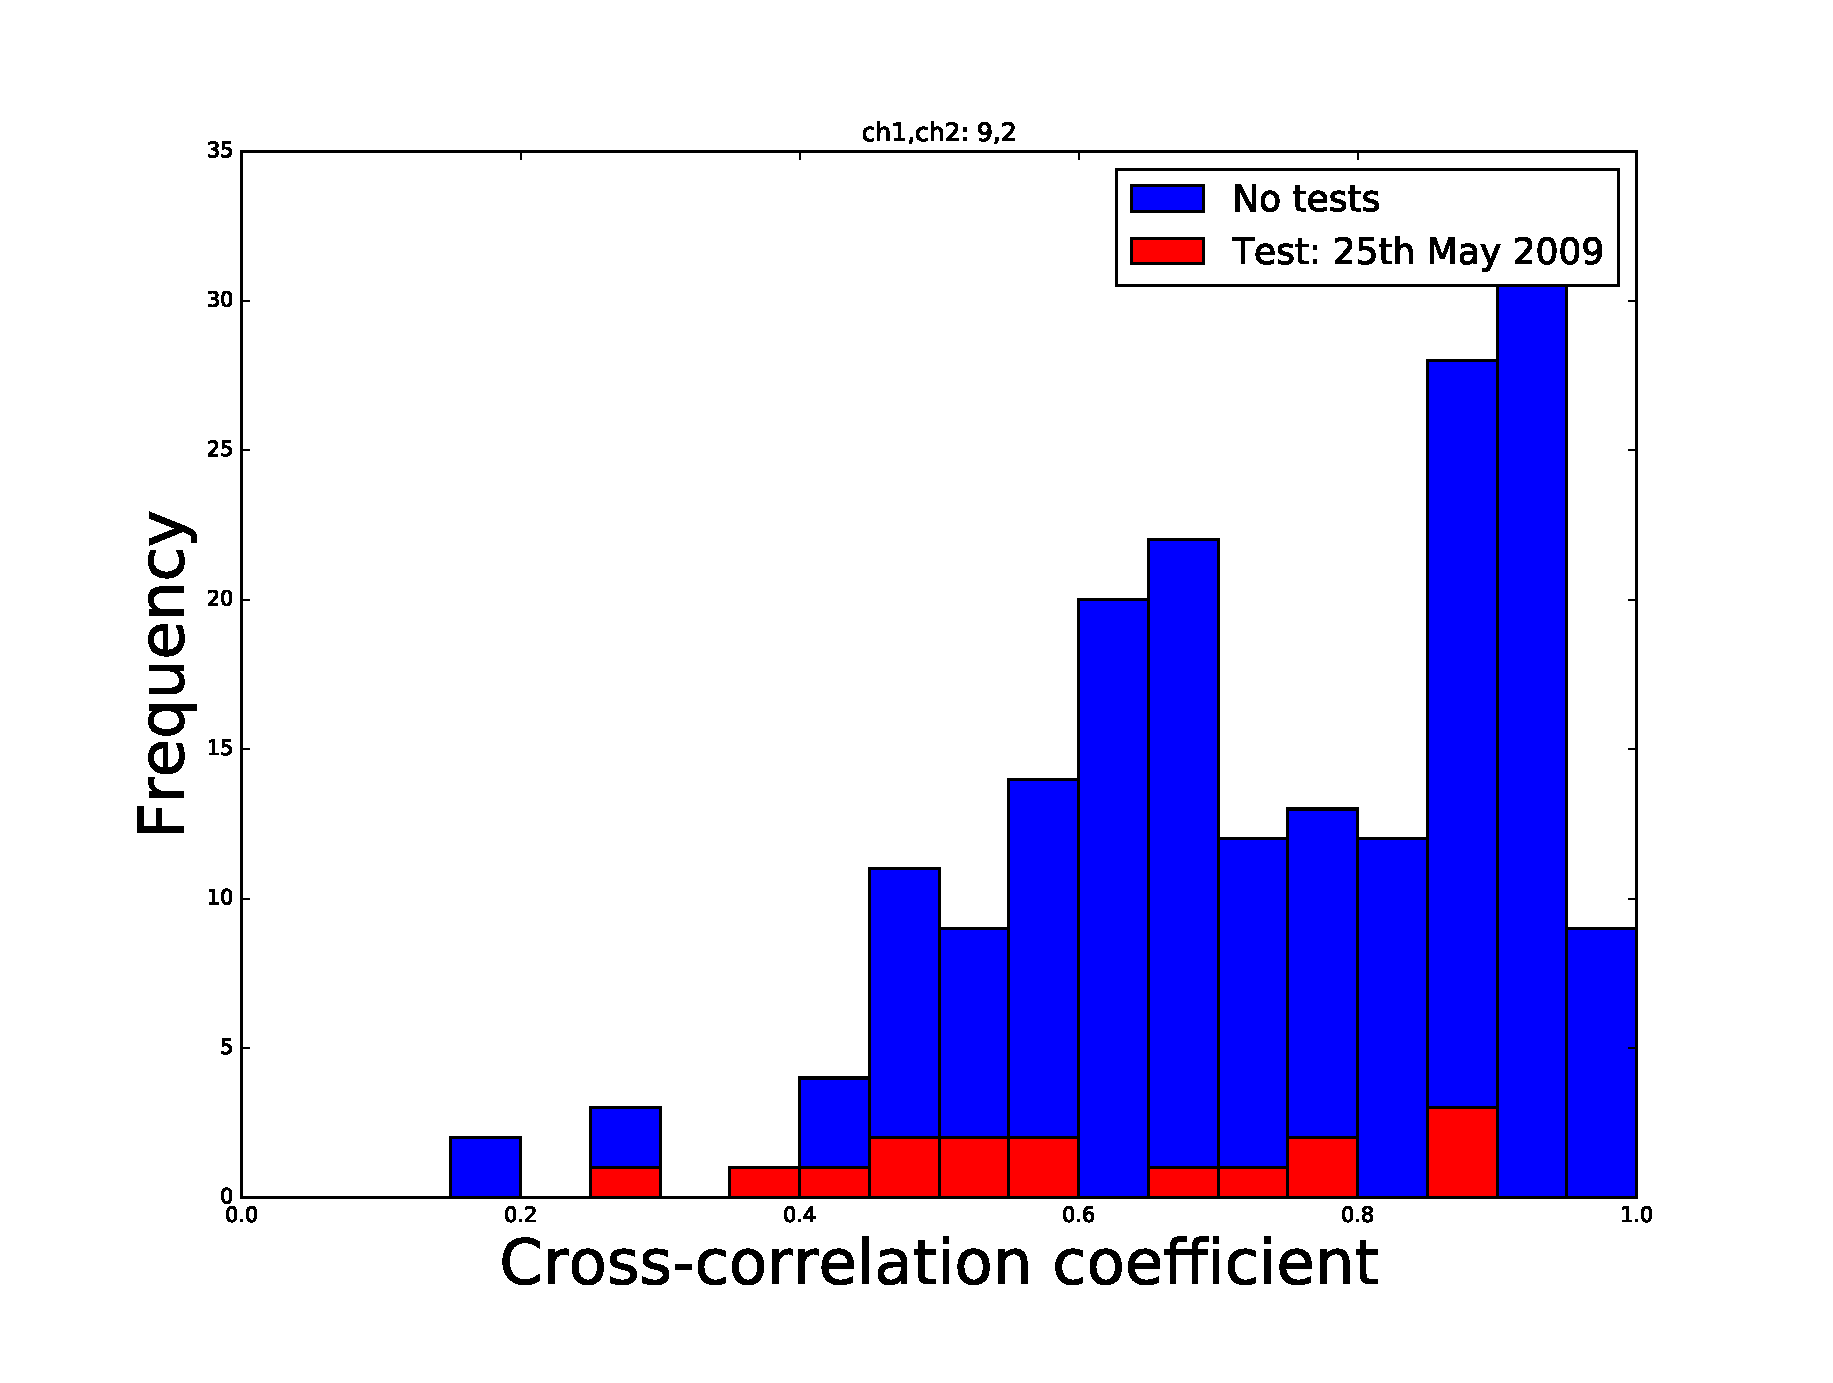
\includegraphics[width=\textwidth]{Figures/eventfind/90hours.eps}
				\caption{90 Hours}
			\end{subfigure}
			\begin{subfigure}[b]{0.5\linewidth}\label{fig:exdatespec}
				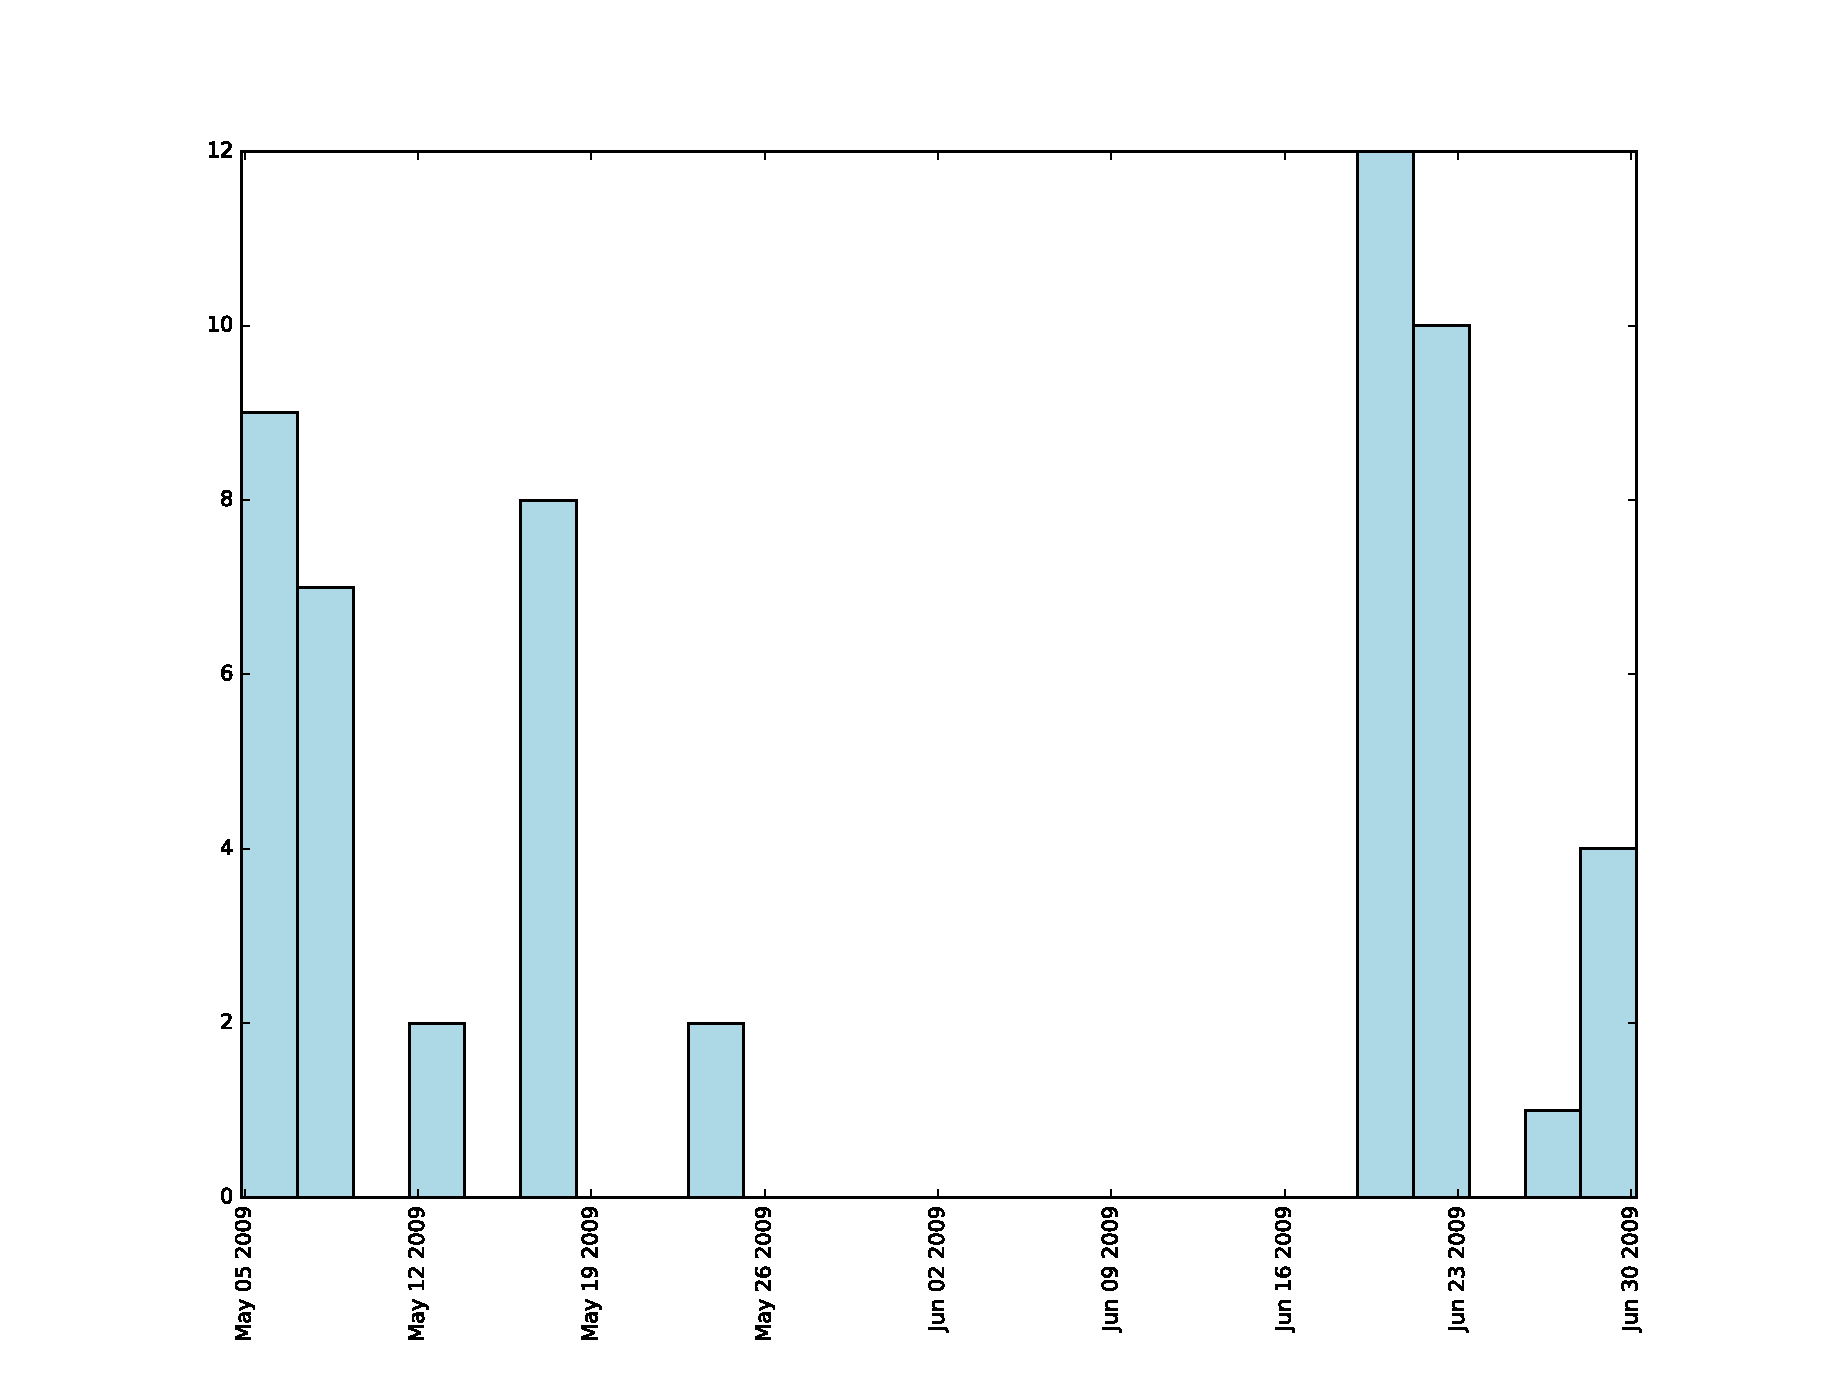
\includegraphics[width=\textwidth]{Figures/eventfind/datespectra.eps}
				\caption{Date spread of lowest cross correlation value for all channels with 90 Hour time intervals}
			\end{subfigure}
			\caption{North Korea Cross correlation spectra for satellite ns\_56 with different}
			\label{fig:tempspecvariation}
		\end{figure}
		Once the adjustments in \secref{ssec:methmod} had been made, we replicate Filip's results by working over a month time period around the North Korea test date to see if the anomalous value intervals clustered around the test date. To observe this specifically, we find the date interval which corresponds to smallest cross correlation in the.
		
		From this you can observe the following:
		\begin{itemize}
			\item
			In \figref{fig:tempspecvariation} and in the majority of the data it can be seen that taking time intervals significantly longer than the expected particle burst mechanism seems to make the North Korea spectra more distinct compared to the background.
			\item
			The dates of the smallest correlation value intervals don't cluster around the test date used, which is a concern.
			\item
			Especially with longer time intervals, the histograms of background seem to have unusual structure larger than a na�ve estimate of the errors on the bins.
			\footnote{This may be less important}
			\item
			For two high energy channels, the cross correlation coefficients tended to be more likely to be close to 1 than the background data.
		\end{itemize}
		\newpage
		\begin{wrapfigure}{R}{0.4\textwidth}
			\caption{Sample 48 hour correlation intervals between channels 2 and 3, two low energy channels on satellite ns\_56}
			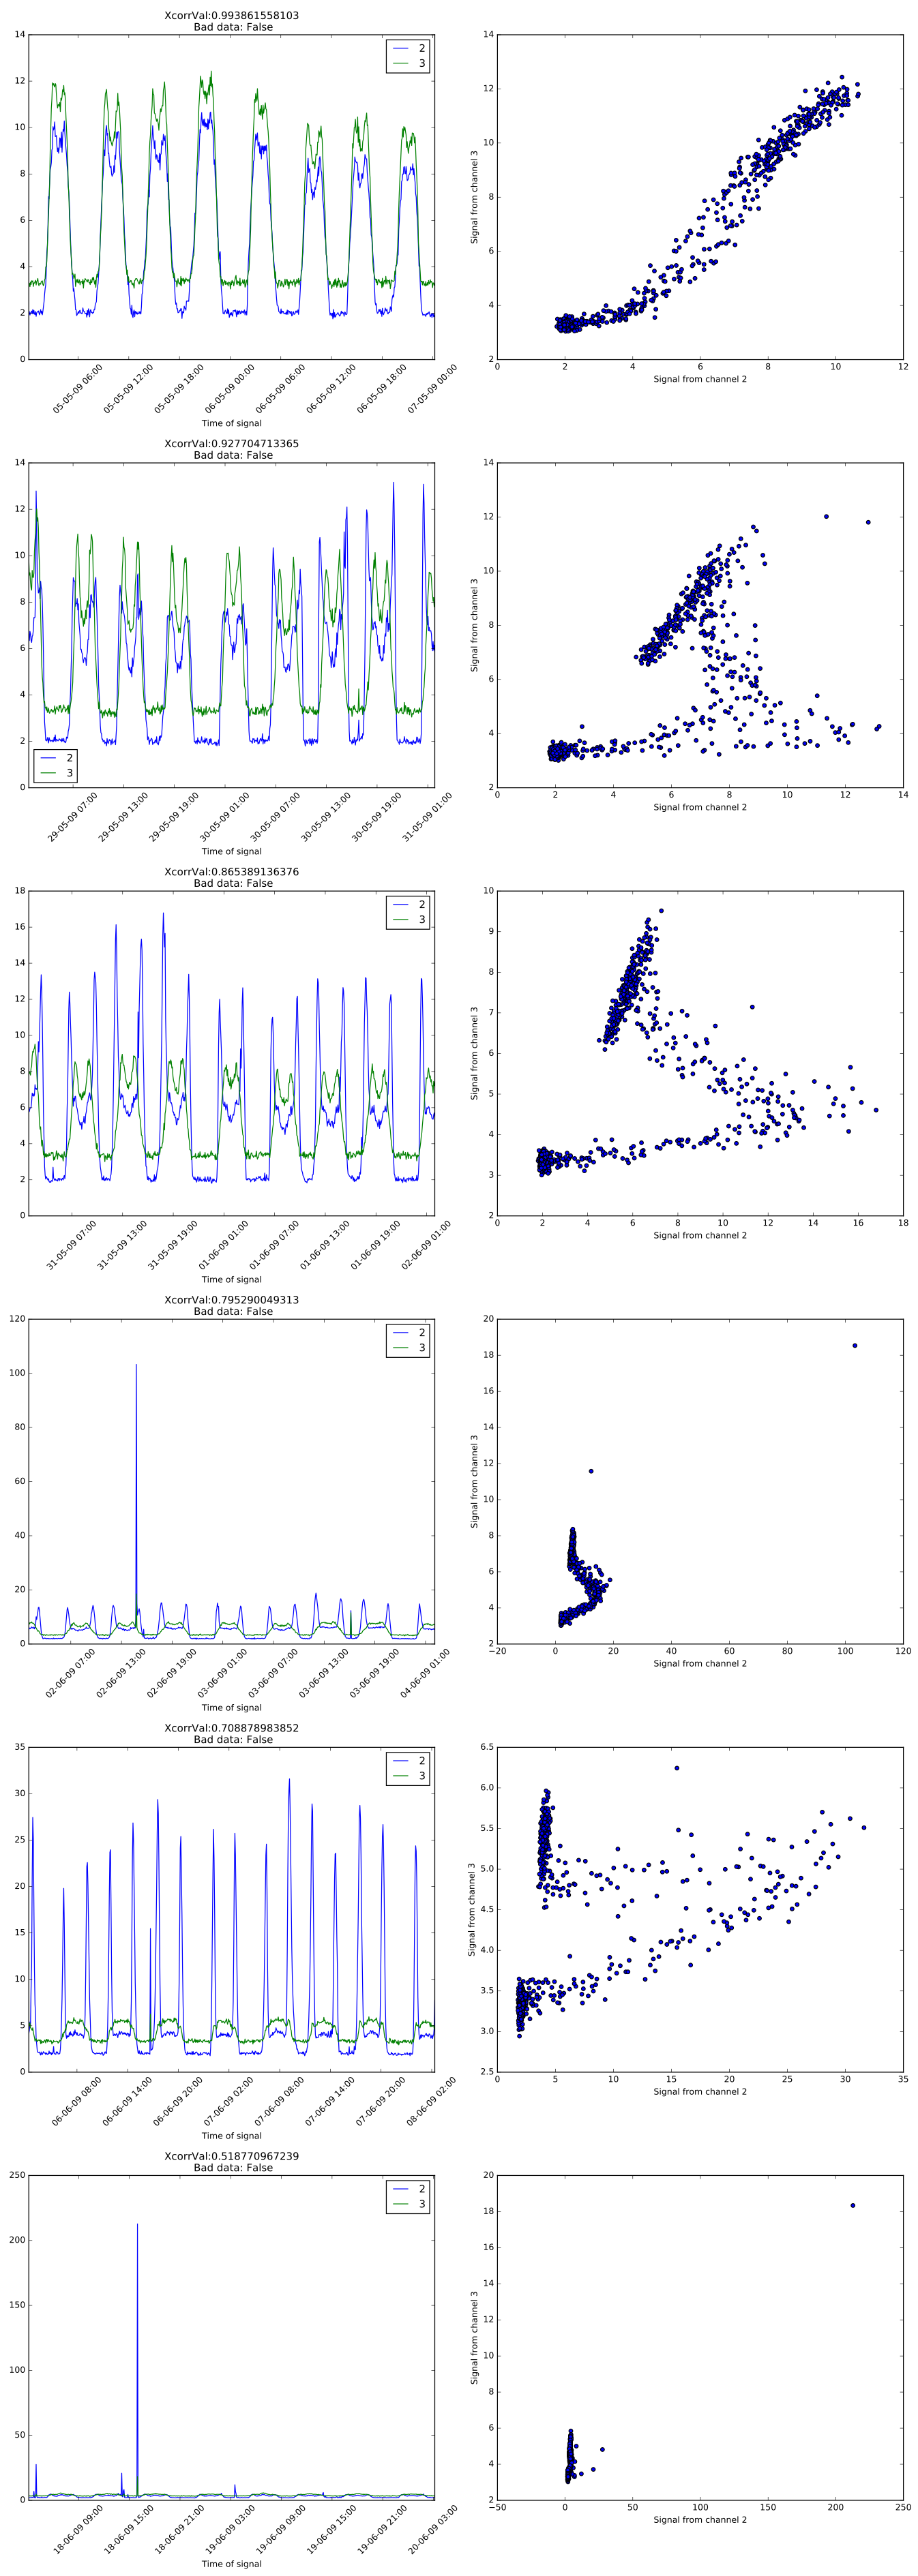
\includegraphics[width=\linewidth]{Figures/2_3}
			\label{fig:2_3}
		\end{wrapfigure}
		\subsubsection{Scatter, Time Series and Fourier transform plots}
		Even though there is no obvious temporal link between the tests and the correlation anomalies, the next logical step was to check the nature of data for the intervals with different correlation coefficients. This allows us to see if smaller/larger cross correlation coefficient values are caused by less correlated data, outliers or non-linear relations between the signals.
		
		Additionally, by creating signal time plots alongside these we can see how structured scatter plots form over time. An example of this is shown in \figref{fig:2_3}
		
		This revealed a large variety of exotic structures which has not been fully analysed but a few things are of note:
		\begin{itemize}
			\item
			Practically all of our plots have a periodic nature and some even seem to have a second periodicity convolved with it. This period seems to be roughly 6 hours but a quick FFT did not produce as clean a signal as one would hope. \footnote{This would be a good way to learn the code}
			\item
			There often seems to be `gaps' in the scatter plot where there is no combination of signals and sometimes form ring-like attractor shapes
			\item
			There are `bursts' of very large signals that can last an hour or so which are not labelled as bad data.
			\item
			Bad data labels often do not break the data as much you'd expect because often bad data just seems to mean that there is no signal (i.e set to 0) for a short period of time
		\end{itemize}
		Furthermore, there is clearly quite a lot still to be analysed in the raw signal alone. However, it seems reasonably clear that just using a cross correlation coefficient to try and classify nuclear test behaviour from background seems unlikely without further metrics and a better understanding of the data.
		\subsubsection{Bad Data Spectra}
		An additional set of plots were created to see if using bad data changed the cross correlation spectra. It seemed that
		%Attach A plot here
\section{Suggestions For Continuation}\label{ssec:suggestions}
\newpage
\bibliographystyle{IEEEtran}
\bibliography{GB_report}
\end{document}